% !TEX root = ../zz-lecture.tex


\chapter{非惯性参考系}
我们首先回忆一下学习牛顿运动定律时涉及的一些概念。牛顿第一定律成立的参考系称为惯性参考系;例如地面以及相对地面静止或匀速直线运动的参考系都是惯性系;牛顿第二定律只在惯性系中成立,在非惯性系中不成立,例如下面这个情景:
静止的火车车厢内有一水平的光滑桌面,桌面上有一个静止的小球;现在使火车突然(相对地面)向左加速,加速度为$ a_s $(规定向左为正方向),这时小球将如何运动呢?

\marginpar{\centering 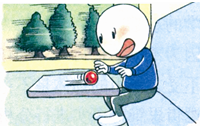
\includegraphics[width=\marginparwidth]{image/NIR-1}\figcaption{突然加速的火车} \label{fig:}}

地面上的观察者发现小球将静止在原地,这是符合牛顿运动定律的;而以车厢为参考系观察会发现小球以$-a_s$相对于车厢做加速运动,小球没有受到水平方向的作用力却产生了加速度,这显然是不符合牛顿运动定律的(实际是牛顿运动定律在这个参考系中不适用)。

\stitle{惯性力}

假设车厢中的人熟知牛顿运动定律,尤其对加速度一定是由力引起的印象至深,以致在任何场合下,他都强烈地要求保留这一认知。
于是车上的人说:小球之所以对小车有加速度$ -a_s $,是因为受到了一个指向右方的作用力,且力的大小为$ ma_s $;物理上把人为引入的$ -ma_s $这个力命名为惯性力。
需要注意的是: 惯性力是一种假想的力,不是物体间的真实相互作用,因此没有施力物体,也没有反作用力。
由于在非惯性系中研究动力学问题有一定难度,因此我们首先研究平动非惯性系的简单情况,对于转动参考系等复杂情况在后面展开。




假设质量为$ m $的物体相对地面的加速度为$ \vec{a} $,所受的合外力为$ \vec{F} $,某参考系S相对地面做平动,加速度为$\vec{a}_s $(即参考系S为非惯性系)。
在地面参考系中,根据牛顿第二定律可得
\[
\vec{F} = m\vec{a}.
\]
根据相对运动的定义,物体$ m $相对参考系S的加速度
\begin{equation}
\vec{a'} = \vec{a}-\vec{a}_s,
\end{equation}
两式联立可得:
\begin{equation}
\vec{F} = m\vec{a}'+m\vec{a}_s,
\end{equation}
将上式稍加变形得到
\begin{equation}
\vec{F}-m\vec{a}_s = m\vec{a}'.
\end{equation}
如果把上式左边$-m \vec{a}_s$看成一个力,(即前面所说的惯性力),我们可以把上式理解成非惯性系中的牛顿第二定律,即在非惯性系中,惯性力与物体所受真实力的合力共同产生物体相对该参考系的加速度。

为了在非惯性系中仍然可以使用牛顿第二定律解决动力学问题,需要对牛顿第二定律做些修正。
在非惯性系中,惯性力与物体所受真实力的合力提供物体的加速度,即
\begin{equation}
\vec{F}+\vec{f}_i = m\vec{a}',
\end{equation}
对于平动非惯性系$ \vec{f}_i = -m\vec{a}_s $(其中$ \vec{a}_s $是非惯性系相对地面的加速度),惯性力的作用点作用在质心上。
需要注意的是对于转动非惯性系,惯性力会比较复杂,可能不止一项。


\begin{example}
	%%%%题干
	若不考虑太阳和其他星体的作用,则地球——月球系统可以看成孤立系统.把地球和月球都看作是质量均匀分布的球体,它们的质量分别为$ M $、$ m $,月心和地心间的距离为$ R $,万有引力常量为$ G $.学生甲以地心为参考系,利用牛顿第二定律和万有引力定律得到月球相对于地心参考系的加速度为$a_m=GM/R^2$ ;学生乙以月心为参考系,同样利用牛顿第二定律和万有引力定律,得到地球相对于月心参考系的加速度为$a_e=Gm/R^2$ .两位同学求出的地月之间的相对加速度大小是不同的,这是不合理的,请定性解释原因.
	%%%%插图
	%	\begin{problemfig}
	%		\includegraphics[width=0.6\linewidth]{image/}
	%	\end{problemfig}
	
	\begin{taggedblock}{student}
		\vspace*{2cm}
	\end{taggedblock}
	
	
	%%%%答案
	\begin{taggedblock}{answer}
		答案:不对。
	\end{taggedblock}
	
	
	%%%%解析
	\begin{taggedblock}{analysis}
		解析:因为地球受到月球的引力作用、月球受到地球的引力作用.它们相对于惯性参考系都有加速度,因此它们都不是惯性参考系.在非惯性系中应用牛顿第二定律时,必须引入惯性力,两位同学都没有引入惯性力,因此算出的结果都是不对的.
	\end{taggedblock}
\end{example}


\begin{example}
	%%%%题干
	 如图所示,被水平拉伸的轻弹簧右端拴在小车壁上,左端拴一质量为\SI{10}{kg} 的物块M.小车静止不动,弹簧对物块的弹力大小为\SI{5}{N}时,物块处于静止状态.当小车向右做加速运动,且加速度逐渐由0增加到\SI{1}{m/s^2}的过程中
	 
	 A. 物块M相对小车仍静止; 
	 
	 B. 物块M受到的摩擦力一直减少; 
	 
	 C. 物体M受到的摩擦力一直增大; 
	 
	 D. 物体M受到的摩擦力先减少后增大.
	 
	 \marginpar{\centering 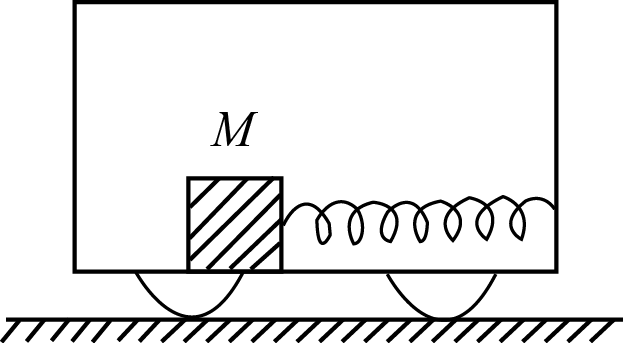
\includegraphics[width=\marginparwidth]{image/NIR-2.png}\figcaption{第\theexample 题} \label{fig:}}
	%%%%插图
	%	\begin{problemfig}
	%		\includegraphics[width=0.6\linewidth]{image/}
	%	\end{problemfig}
	
	\begin{taggedblock}{student}
		\vspace*{2cm}
	\end{taggedblock}
	
	
	%%%%答案
	\begin{taggedblock}{answer}
		答案:AD
	\end{taggedblock}
	
	
	%%%%解析
	\begin{taggedblock}{analysis}
		解析: 引入惯性力的概念,此时相当于给物体增加了一个水平向左的惯性力,而且此力的大小从0开始逐渐增大到\SI{10}{N} ,按照题中条件,摩擦力可以达到\SI{5}{N},因此物体始终与小车相对静止.摩擦力先减小再反向增大.
	\end{taggedblock}
\end{example}



\begin{example}
	%%%%题干
	如图,水平地面上有一楔形物体b,b的斜面上有一小物块a;a与b之间、b与地面之间均存在摩擦.已知楔形物体b静止时,a静止在b的斜面上.现给a和b一个共同的向左的初速度,与a和b都静止时相比,此时可能
	
	A.a与b之间的压力减少,且a相对b向下滑动
	
	B.a与b之间的压力增大,且a相对b向上滑动
	
	C.a与b之间的压力增大,且a相对b静止不动
	
	D.  b与地面之间的压力不变,且a相对b向上滑动
	
	\marginpar{\centering 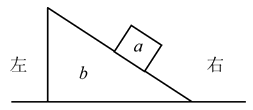
\includegraphics[width=\marginparwidth]{image/NIR-3}\figcaption{第\theexample 题} \label{fig:}}
	%%%%插图
	%	\begin{problemfig}
	%		\includegraphics[width=0.6\linewidth]{image/}
	%	\end{problemfig}
	
	\begin{taggedblock}{student}
		\vspace*{2cm}
	\end{taggedblock}
	
	
	%%%%答案
	\begin{taggedblock}{answer}
		答案:BC
	\end{taggedblock}
	
	
	%%%%解析
	\begin{taggedblock}{analysis}
		解析:本题同样可以在地面参考系中分析,但由于存在多种可能性,讨论起来比较复杂.下面我们以b为参考系,借助惯性力来分析.
		\marginpar{\centering 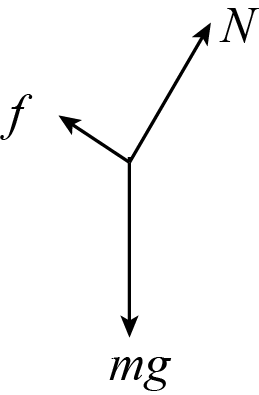
\includegraphics[width=0.6\marginparwidth]{image/NIR-4.png} }
		首先,a、b均静止时,在地面参考系中可知a受到重力$ mg $、支持力$ N $、摩擦力$ f $保持平衡,如图所示.
		当a、b向左运动时,由于地面存在摩擦力,因此b应有向右的加速度,做减速运动,以b为参考系,物块a的受力应增加一个水平向左的惯性力.在此参考系中,物块a在垂直斜面方向没有加速度,由平衡条件可知,支持力$ N $一定增大.在沿斜面方向分析可知:摩擦力可以减小或反向增大,因此,物块a可能继续保持静止或沿斜面向上滑动,但绝不可能沿斜面向下滑动(因为原来的静摩擦力小于最大静摩擦力),BC正确.
		
	\end{taggedblock}
\end{example}


\begin{example}
	%%%%题干
	如图所示,汽车内固定有一个倾角为$ \deg{37} $的斜面,斜面表面光滑,底部有一个质量为$ m $的小物块,开始时系统静止,某时刻汽车突然开始向左以加速度$ a $做匀加速运动.要使物体沿斜面向上运动,则$ a $至少多大.
	\marginpar{\centering 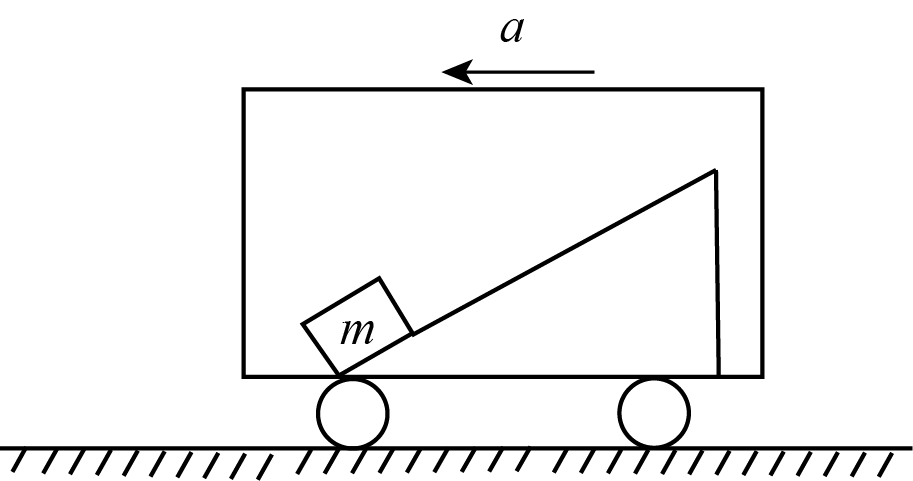
\includegraphics[width=\marginparwidth]{image/NIR-5.png}\figcaption{第\theexample 题} \label{fig:}}
	%%%%插图
	%	\begin{problemfig}
	%		\includegraphics[width=0.6\linewidth]{image/}
	%	\end{problemfig}
	
	\begin{taggedblock}{student}
		\vspace*{2cm}
	\end{taggedblock}
	
	
	%%%%答案
	\begin{taggedblock}{answer}
		答案:$ a>\frac{3}{4}g $
	\end{taggedblock}
	
	
	%%%%解析
	\begin{taggedblock}{analysis}
		解析:以斜面为参考系,物块受到水平向右的力$ F=ma $作用,要使物块沿斜面向上运动,则沿斜面方向$ F\cos\theta-mg\sin\theta>0 $,解得$a>3/4 g$.
	\end{taggedblock}
\end{example}


\begin{example}
	%%%%题干
	 质量为 $ M $的楔子置于光滑水平面上,给楔子施加水平推力 $ F $,要使质量为 $ m $的小球沿其倾角 $ \alpha $的粗糙斜面向上滚动,求$ F $的最小值。
	%%%%插图
	%	\begin{problemfig}
	%		\includegraphics[width=0.6\linewidth]{image/}
	%	\end{problemfig}
	
	\begin{taggedblock}{student}
		\vspace*{1cm}
	\end{taggedblock}
	
	
	%%%%答案
	\begin{taggedblock}{answer}
		答案:$ (M+m)g\tan\alpha $
	\end{taggedblock}
	
	
	%%%%解析
	\begin{taggedblock}{analysis}
		解析:当球刚好要沿斜面向上滚动时 $ F $有最小值,此时,对整体有: $ F=(M+m)a $.
		在斜面参考系中,球刚好能滚动,因此以球和斜面接触点为轴,小球所受力矩平衡,有: 
		\[
		mar\cos\alpha = mgr\sin\alpha,
		\]
	联立解得: $F=(M+m)g\tan\alpha⁡$.
		
	\end{taggedblock}
\end{example}


\begin{example}
	%%%%题干
	 一辆汽车质量为$ m $,前后轮相距$ 2l $,质心在车辆中心、距地面高度为$ h $.初始时车辆在平直路面做匀速直线运动,突然遇到紧急情况急刹车停下,为保证车辆不向前翻倒,则刹车过车中加速度最大为多少(地面摩擦因数足够大,不考虑车辆滑动)
	 \marginpar{\centering 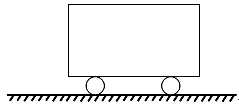
\includegraphics[width=0.8\marginparwidth]{image/NIR-6.png}\figcaption{第\theexample 题} }
	%%%%插图
	%	\begin{problemfig}
	%		\includegraphics[width=0.6\linewidth]{image/}
	%	\end{problemfig}
	
	\begin{taggedblock}{student}
		\vspace*{2cm}
	\end{taggedblock}
	
	
	%%%%答案
	\begin{taggedblock}{answer}
		答案:$\frac{gl}{h}$
	\end{taggedblock}
	
	
	%%%%解析
	\begin{taggedblock}{analysis}
		解析:略
	\end{taggedblock}
\end{example}



\begin{example}
	%%%%题干
	 如图所示,在以一定加速度$ a $行驶的车厢内,有一长为$ l $,质量为$ m $的棒AB靠在光滑的后壁上,棒与车箱底之间的动摩擦因数为$ \mu $.为了使棒不滑动,棒与竖直平面所成的夹角$ \theta $应在什么范围内?
	 \marginpar{\centering 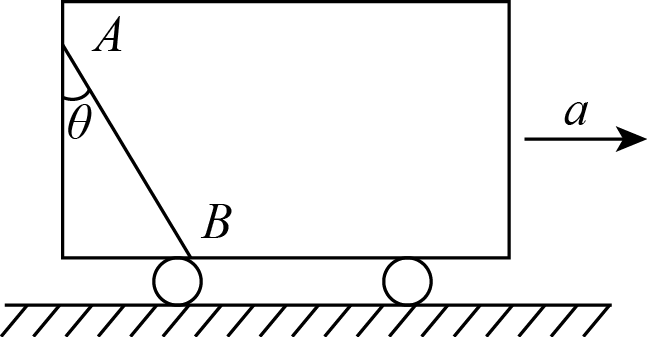
\includegraphics[width=\marginparwidth]{image/NIR-7.png}\figcaption{第\theexample 题} \label{fig:}}
	%%%%插图
	%	\begin{problemfig}
	%		\includegraphics[width=0.6\linewidth]{image/}
	%	\end{problemfig}
	
	\begin{taggedblock}{student}
		\vspace*{2cm}
	\end{taggedblock}
	
	
	%%%%答案
	\begin{taggedblock}{answer}
		答案:$ \arctan\frac{a-2\mu g}{g}\le \theta \le \arctan\frac{a+2\mu g}{g} $
	\end{taggedblock}
	
	
	%%%%解析
	\begin{taggedblock}{analysis}
		\marginpar{\centering 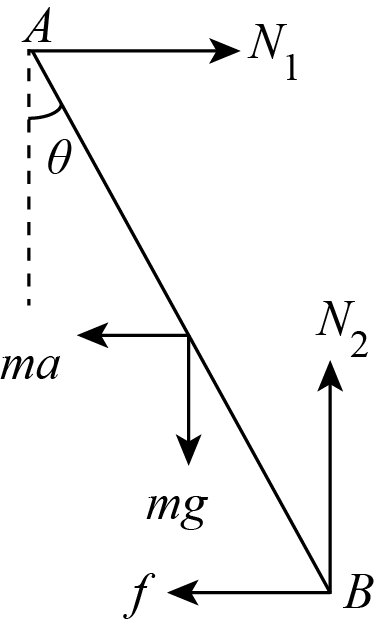
\includegraphics[width=0.6\marginparwidth]{image/NIR-8}}
		解析:以车厢为参照系,惯性力的作用点在棒的重心处,
		当$ \theta $取最大值时,棒AB刚好不滑动,受力如图所示,此时B端所受摩擦力的方向水平向左,且达最大静摩擦力,
		以A点为轴,由力矩平衡条件得
		\[
		ma\frac{l}{2}\cos\theta+fl\cos\theta+mg\frac{l}{2}\sin\theta = N_2l\sin\theta,
		\]
		又由受力平衡条件得:$N_2=mg$,$		f=\mu N_2$,解得
		\[
		\theta_{max} = \arctan\frac{a+2\mu g}{g}.
		\]
		同理,当$ \theta $取最小值时,棒的B端所受摩擦力方向水平向右,
		由力矩平衡条件得:
		\[
			ma\frac{l}{2}\cos\theta+mg\frac{l}{2}\sin\theta = N_2l\sin\theta+fl\cos\theta,
		\]
	可解得$ θ_{min}=arctan⁡(a-2μg)/g $,综上所述,要使棒不滑动,应满足$ \arctan\frac{a-2\mu g}{g}\le \theta \le \arctan\frac{a+2\mu g}{g} $。
		
		
	\end{taggedblock}
\end{example}


\begin{example}
	%%%%题干
	如图所示,质量为$ m $的物体放置在倾角为$ \alpha $的斜面上,且用绳连接在墙上,不计一切摩擦,当斜面以加速度$ a $向右运动时,求绳上的拉力.
	\marginpar{\centering 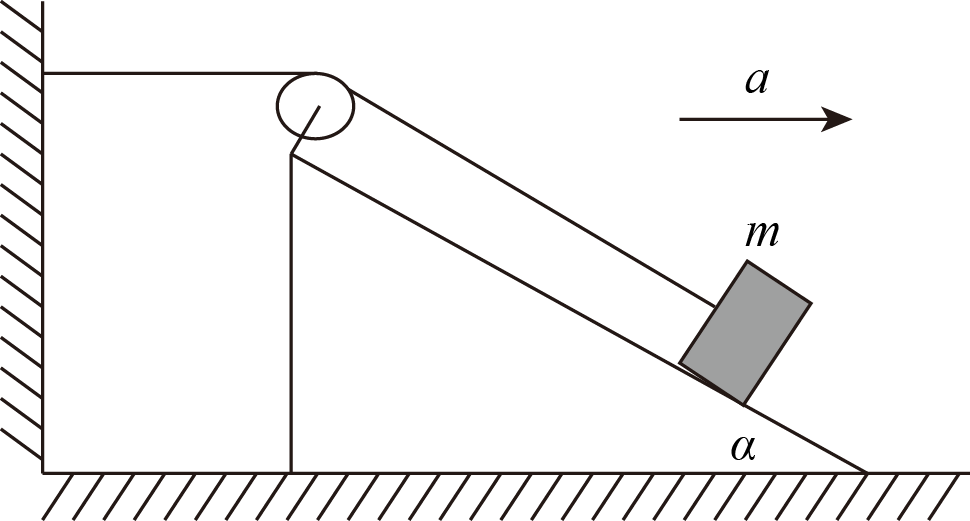
\includegraphics[width=\marginparwidth]{image/NIR-9.png}\figcaption{第\theexample 题} \label{fig:}}
	%%%%插图
	%	\begin{problemfig}
	%		\includegraphics[width=0.6\linewidth]{image/}
	%	\end{problemfig}
	
	\begin{taggedblock}{student}
		\vspace*{2cm}
	\end{taggedblock}
	
	
	%%%%答案
	\begin{taggedblock}{answer}
		答案:$ ma-ma\cos\alpha+mg\sin\alpha $
	\end{taggedblock}
	
	
	%%%%解析
	\begin{taggedblock}{analysis}
			\marginpar{\centering 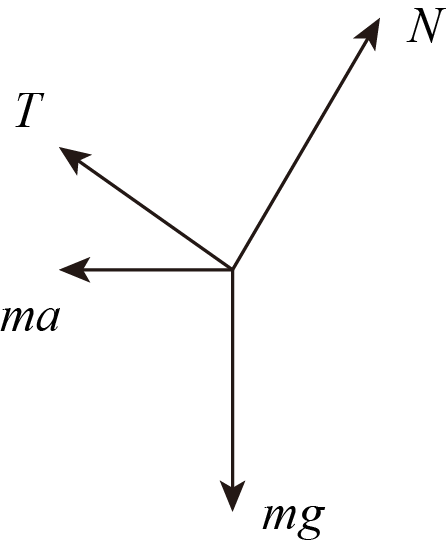
\includegraphics[width=0.6\marginparwidth]{image/NIR-10}}
		解析:本题在地面参考系中研究,$ m $的运动比较复杂,求解有一定难度,因此我们以斜面为参考系考虑这个问题;
		以斜面为参考系,物体受到重力$ mg $、支持力$ N $、拉力$ T $、惯性力$ ma $,如图所示,墙相对斜面以加速度$ a $拉绳子,所以物体沿斜面方向的加速度大小也是$ a $;
		沿斜面方向应用牛顿第二定律得:
		\[
		T+ma\cos\alpha-mg\sin\alpha=ma
		\]
		解得:$ T=ma-ma\cos\alpha+mg\sin\alpha $⁡α.
	
		
	\end{taggedblock}
\end{example}


\begin{example}
	%%%%题干
	 如图所示,与水平面成$ \theta $角的光滑棒AB上有一滑套C,开始时与棒的A端相距为$ l $,相对棒静止.当棒保持倾角$ \theta $不变沿水平面匀加速运动,加速度为$a(a>g\tan\theta)$时,求滑套C从棒的A端滑出所经历的时间.
	 	\marginpar{\centering 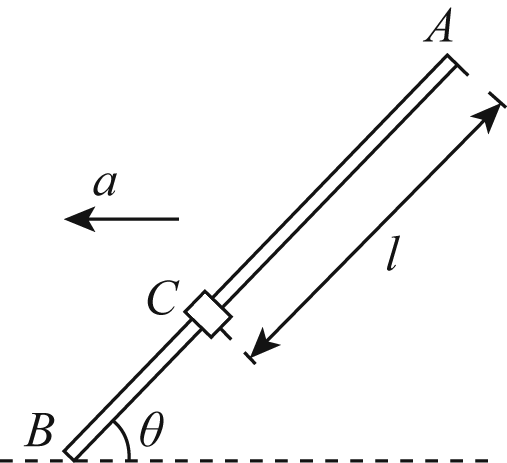
\includegraphics[width=\marginparwidth]{image/NIR-11.png}\figcaption{第\theexample 题} \label{fig:}}
	%%%%插图
	%	\begin{problemfig}
	%		\includegraphics[width=0.6\linewidth]{image/}
	%	\end{problemfig}
	
	\begin{taggedblock}{student}
		\vspace*{2cm}
	\end{taggedblock}
	
	
	%%%%答案
	\begin{taggedblock}{answer}
		答案:$ \sqrt{\frac{2l}{a\cos\theta-g\sin\theta}} $.
	\end{taggedblock}
	
	
	%%%%解析
	\begin{taggedblock}{analysis}
		\marginpar{\centering 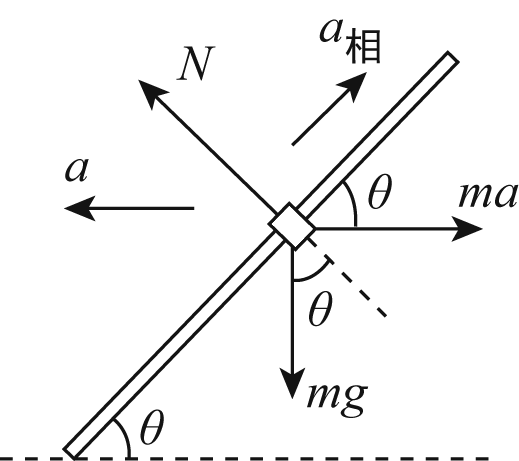
\includegraphics[width=0.8\marginparwidth]{image/NIR-12.png}}
		解析:以棒为参照系,对滑套C受力分析如图所示,
			由牛顿第二定律有
			\[
			ma\cos\theta-mg\sin\theta = ma_r,
			\]
		滑套相对杆做匀加速直线运动,由运动学公式
		\[
		l = \frac{1}{2}a_rt^2,
		\]
		联立解得
		\[
		t = \sqrt{\frac{2l}{a\cos\theta-g\sin\theta}} 
		\]
		
	\end{taggedblock}
\end{example}



\begin{example}
	%%%%题干
	在光滑的水平面上有一质量为$ M $、倾角为$ \theta $的光滑斜面,其上有一质量为$ m $的物块,如图所示.求物块在下滑的过程中对斜面压力的大小。
		 	\marginpar{\centering 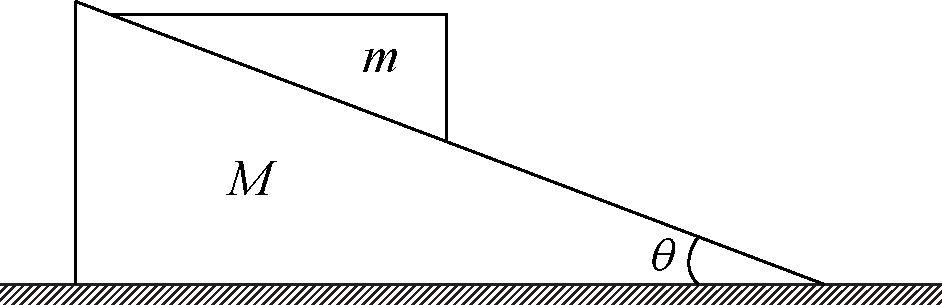
\includegraphics[width=\marginparwidth]{image/NIR-13.png}\figcaption{第\theexample 题} \label{fig:}}
	%%%%插图
	%	\begin{problemfig}
	%		\includegraphics[width=0.6\linewidth]{image/}
	%	\end{problemfig}
	
	\begin{taggedblock}{student}
		\vspace*{2cm}
	\end{taggedblock}
	
	
	%%%%答案
	\begin{taggedblock}{answer}
		答案:
	\end{taggedblock}
	
	
	%%%%解析
	\begin{taggedblock}{analysis}
		\begin{center}
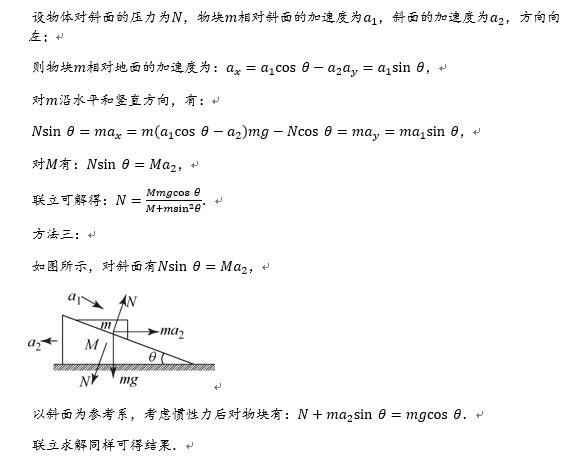
\includegraphics[width=0.9\linewidth]{image/NIR-14}
\end{center}

		
	\end{taggedblock}
\end{example}

\begin{example}
	%%%%题干
	如图所示,光滑的直角三角形斜楔C,质量不计,放置在光滑水平地面上,两侧各自放一个质量为$ m $的物块A、B,静止释放,计算释放后C的加速度.
			 	\marginpar{\centering 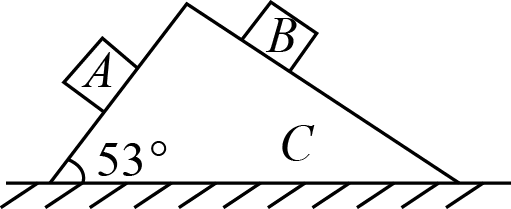
\includegraphics[width=\marginparwidth]{image/NIR-15.png}\figcaption{第\theexample 题} \label{fig:}}
	%%%%插图
	%	\begin{problemfig}
	%		\includegraphics[width=0.6\linewidth]{image/}
	%	\end{problemfig}
	
	\begin{taggedblock}{student}
		\vspace*{2cm}
	\end{taggedblock}
	
	
	%%%%答案
	\begin{taggedblock}{answer}
		答案:$ a=0 $
	\end{taggedblock}
	
	
	%%%%解析
	\begin{taggedblock}{analysis}
				\begin{center}
					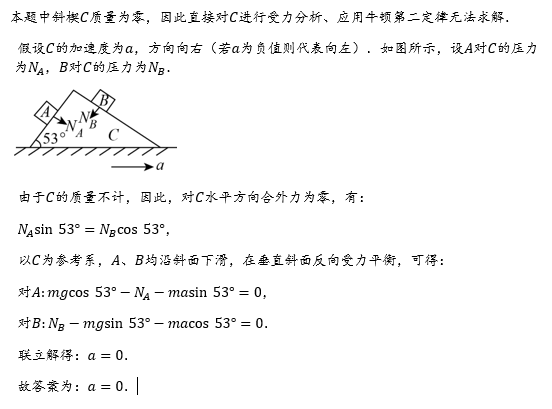
\includegraphics[width=0.9\linewidth]{image/NIR-16}
				\end{center}
	\end{taggedblock}
\end{example}